\section{Contributions}
\begin{frame}{Contributions}

    The paper addresses the problem of \gbf{fairness} in \gbf{bipartite ranking models}, which have different requirements than classification models.
    
    The authors came up with \gbf{two contributions} to \gbf{improve fairness} of bipartite ranking models :
  \begin{itemize}
      \item AUC-based constraints
      \item ROC-based constraints
  \end{itemize}
  
  They show the \gbf{limitations} of the AUC-based constraints, and how the ROC-based constraints \gbf{address} them.
\end{frame}

\begin{frame}{Motivation}
    \begin{itemize}
        \item The vast majority of fairness-aware machine learning research focuses on classification models.
        \item However, many real-worl applications require bipartite ranking models. 
        \item Because they are evaluated differently (\textit{i.e}, with ROC curves), evaluating fairness for bipartite ranking models might also be more challenging.        
        \item However, learning a scoring function over a classifier adds more flexibility to the thresholds, which means that a fair scoring function will lead to fair decisions for all thresholds of interest.
    \end{itemize}
\end{frame}


\subsection{AUC-based constraints}
\begin{frame}{AUC-based constraints}

\end{frame}

\begin{frame}{Limits of AUC-based constraints}
    \begin{figure}[t]
        \centering
        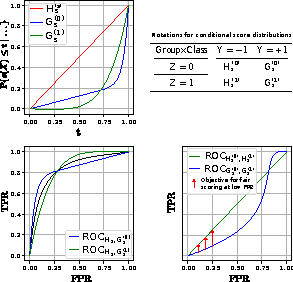
\includegraphics[width=0.6\columnwidth]{images/original_paper/example_simple_dists_explained_with_table2.pdf}
        \caption{Illustrating the limitations of $AUC$-based fairness.}
        \label{fig:example-1}
    \end{figure}
\end{frame}

\subsection{ROC based constraints}
\begin{frame}{ROC based constraints}
    small change another change final change hopefully ok now it works
\end{frame}
